\documentclass{article}
\usepackage[final]{nips_2017}
\usepackage[utf8]{inputenc} % allow utf-8 input
\usepackage[T1]{fontenc}    % use 8-bit T1 fonts
\usepackage{hyperref}       % hyperlinks
\usepackage{url}            % simple URL typesetting
\usepackage{booktabs}       % professional-quality tables
\usepackage{amsfonts}       % blackboard math symbols
\usepackage{nicefrac}       % compact symbols for 1/2, etc.
\usepackage{microtype}      % microtypography
\usepackage{graphicx}
% \usepackage{multicol}
\usepackage{wrapfig}
\graphicspath{ {./images/} }

\title{In-depth: Depth Map Estimation From Monocular RGB Image Using Deep Learning}

\author{
  Xu Guo\\
  Stanford University\\
  \texttt{xuguo@stanford.edu}\\
  %% examples of more authors
  \And
  Isha Singhal\\
  Stanford University\\
  \texttt{isha22@stanford.edu}\\
  \And
  Meijiao Png\\
  Stanford University\\
  \texttt{mpng@stanford.edu}\\
  %% Coauthor \\
  %% Affiliation \\
  %% Address \\
  %% \texttt{email} \\
  %% \AND
  %% Coauthor \\
  %% Affiliation \\
  %% Address \\
  %% \texttt{email} \\
  %% \And
  %% Coauthor \\
  %% Affiliation \\
  %% Address \\
  %% \texttt{email} \\
  %% \And
  %% Coauthor \\
  %% Affiliation \\
  %% Address \\
  %% \texttt{email} \\
}


\begin{document}

    \begin{center}
    
\includegraphics[width=3cm, height=0.7cm]{CS230}
    \end{center}

    \maketitle

% \begin{multicols}{2}
\begin{abstract}
    This report addresses the approaches of predicting depth from a single RGB image. Our implementation is based on the approaches presented by Eigen et al. \cite{nips-1} based on a two pass CNN model.  This code is made available on Github \cite{github-repo}. We evaluate the outcomes of our approaches in defined metrics and loss value. We also present several directions that we experimented in the project, such as data augmentation, batch normalization, dropout, and network architecture changes.
\end{abstract}

\section{Introduction}	
    RGB-D images augment conventional RGB images with additional depth information on a per-pixel basis. This additional information can be used in various applications that include 3D reconstruction, AR/VR and image processing.  

    While modern consumer technology such as smartphones have enabled more people to take RGB photos, it is still difficult to obtain RGB-D images. There has been numerous efforts in industry to integrate specialized sensors into hardware to capture depth information (Google Project Tango, lenovo Phab2 pro, intel realsense). However, the efforts have not been successful because depth sensing capabilities require extra hardware, accurate calibration and extra design space. It is usually hard to justify the large BOM cost (bill of material cost), production line change, and drastic industrial design change of the phone to incorporate depth sensors.
    
    In this paper, we evaluate deep learning approaches to construct “application ready” depth image using a single RGB camera image, which leapfrogs the need of specialized depth sensor.
    
\section{Related Work}
    Our approach implements the research from Eigen et. al\cite{nips-1}, described in section 3.2. Prior to Eigen et. al\cite{nips-1}, there were approaches that estimate depth from a single image such as in Saxena et. al\cite{pp5} but relies on alignment of several images for the same scene.  Karsch et al\cite{pp7} used a kNN transfer mechanism that is augmented with motion information, which also requires expensive alignment procedures. Newer approaches include the use of Generative Adversarial Networks by Tan et. al\cite{pp6} that has an encoder-decoder type generator with residual transposed convolution blocks trained with an adversarial loss. 

\section{Dataset and Preprocessing}
    
\begin{wrapfigure}{R}{0.35\textwidth}
    \centering
    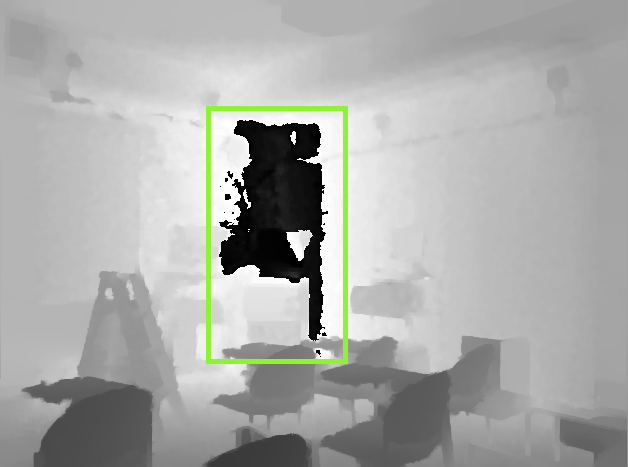
\includegraphics[width=0.35\textwidth]{images/depth_with_invalid.png}
    \caption{depth image with invalid depth, area circled in green}
    \label{fig:invalid_depth}
\end{wrapfigure}
    
    Our dataset comes from NYU Depth dataset \cite{nyu_dataset} which contains 1449 pairs of RGBD images of indoor scenes recorded by Microsoft Kinect. Although the dataset contains information including segmentation, object label, etc, our training only takes two sections of the data: depth and image.

    Color image data consist of 3 RGB channels with uint8 integers, depth image consists of a single channel float point data representing real world distance measured in meters. In the preprocessing step, the RGB channels data are normalized to [0.0, 1.0], while the depth value are kept as is. The normalization of depth value did not improve either the estimation accuracy or the learning velocity, thus the depth value are unprocessed to simplify the metric computation.
    
    Due to the limitation of the depth capturing hardware, the NYU depth dataset’s ground contain a number of examples that have invalid depth point, where its depth pixel value is 0.0 (as shown in Figure \ref{fig:invalid_depth}). These invalid depth areas are usually due to black or reflective surface in the scene. When computing the loss, these points are ignored to avoid the invalid value contributing to the overall loss.
    
    The preprocessing step also performs data augmentation to the 1449 RGB-D pairs. To avoid the blank areas caused by shifting and rotation of image, we only deployed three types of augmentation: 1. Scale. 2. Brightness change 3. Horizontal flip. 

    Scale factors are set to be uniformly distributed from 0.7 to 1.0, and brightness are between 0.8 to 1.0. These augmentation parameters are set to be not so large to maintain the original color and structure of the objects captured in the scene. When scaling the image, the depth value in the depth image are proportionally scaled down to maintain the real world distance for the depth.

    The final step preprocessing pipeline downscale the image to the proper size to the network, as well as downscale the depth image to the output size of the network. The downscale step was done using nearest neighbor algorithm. The final output of color image dimension is (1449, 228, 304, 3), the final output of depth image dimension is (1449, 55, 74, 1).
    
    As the project is largely for experimental and learning, we split our dataset to train 90/ dev 10 without test set split, which has 1,304 in training and 145 in dev. Given that the NYU dataset we have are largely indoor and captured in similar house or office sets, the train and dev data maintains the same distribution by default.

\section{Architecture}
    Similar to the approach Eigen et al \cite{nips-1}, we started with a coarse-scale network to achieve a global view of the scene. This is needed to make use of broader cues such as vanishing points and object angles, and high contrast edges. The output of the coarse scale network was then fed to a fine-scale network to obtain local refinements, keeping the coarse scale output fixed with no back-propagation through the coarse layers. All layers use ReLU for activation except for the final layer, which is linear to obtain the target depth. We have used Batch Normalization at every layer to reduce covariant shift. Also, we have added dropout at every layer, starting with 0.1 dropout rate at the first layer and gradually increasing it to 0.5 for the last layer. 
    
    Within the coarse-scale network, there were 5 feature extraction layers followed by 2 fully connected layers. For the fine-scale network, we have only convolution layers with the exception of the first stage to obtain layer edge features.

\begin{figure}[t]
    \centering
    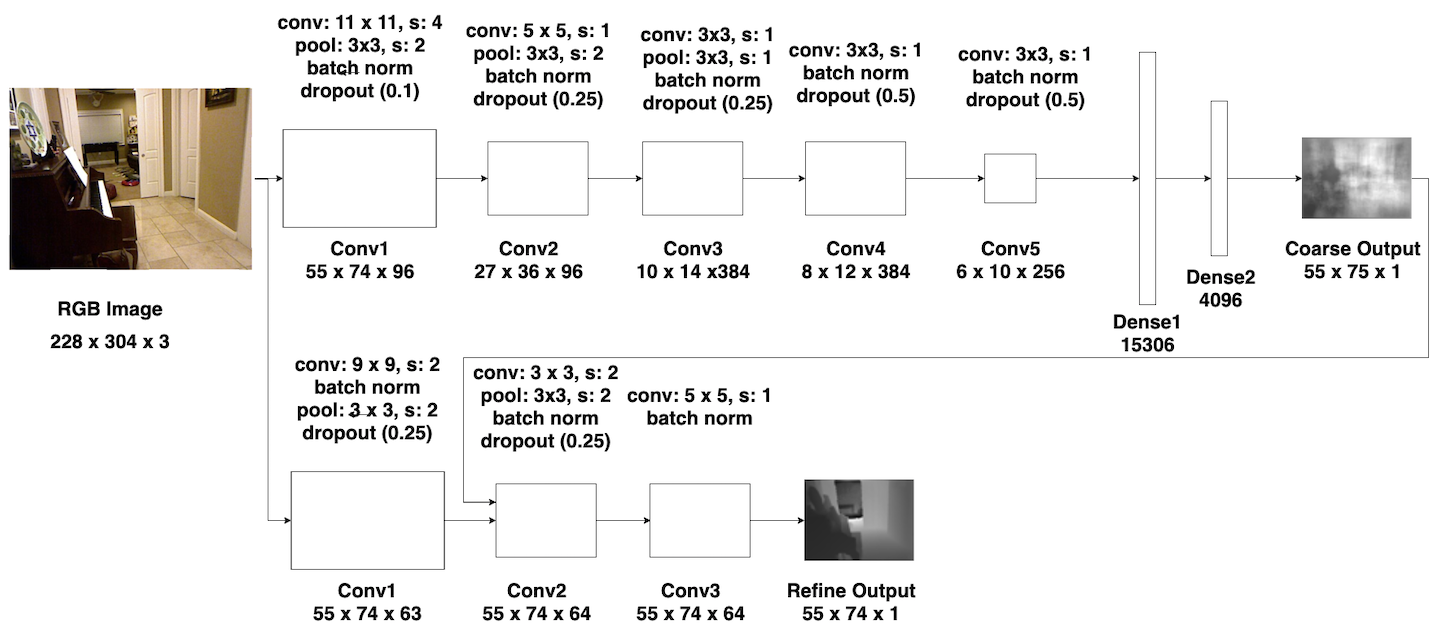
\includegraphics[width=1.0\textwidth]{images/arch-full.png}
    \caption{Model Architecture}
    \label{fig:arch-full}
\end{figure}

\section{Loss Function}
    We used scale invariant loss error to optimize our model, which normalizes differences in room and object sizes. The intuition is that the network is good at figuring out relative positions for an object within the scene, e.g table is in front of TV. However, it is challenging for the network to find out how much in absolute depth an object is away from each other. 
    
    The loss function is defined as below, It is referenced in the paper \cite{nips-1}:
\begin{equation}
    L(y, \hat{y}) = 1/n \sum d_{i}^{2} + \lambda/n^2 (\sum d_{i})^2 , 
    \lambda\in [0, 1]
\end{equation}

\begin{equation}
    d = log(y^{i}) - log(\hat{y}^{i})
\end{equation}

    The loss function has an extra term $1/n^2 (di)^2$ that credits mistakes if they are in the same direction and penalizes them if they oppose. Thus, an imperfect prediction will have lower error when its mistakes are consistent with one another. Setting $\lambda = 0$ reduces to element-wise error, while $\lambda = 1$ is the scale-invariant error exactly.
    
    In our training, we have set $\lambda = 1$ and used the loss as the mean of losses over the batch size. During training, most of the target depth maps will have some missing values, particularly near object boundaries, windows and specular surfaces. We deal with these simply by masking them out, and evaluating the loss only on valid points. Also during training, some of the output values might reach infinity values, we cap these infinity values to 10 to avoid exponential gradients problem. According to the dataset and our assumption, 10 is the maximum absolute distance that could be reached in the depth map image.


\section{Training}
    We split our dataset into 90\% for the training set and 10\% in the test set with a total of 1440 images for the baseline model. We then split the images into mini batches of 32 images.
    We used two pass training method for training our models i.e. we first trained the coarse model and then kept the coarse model weights fixed to train the refine model. 
    
    Initial results showed that our model suffered from high variance, with validation loss above training loss (shown in figure \ref{fig:loss-curve}). This indicated that our model was overfitting the training set. The predicted images confirmed our thoughts, with a poorer outcome when predicting an image from the dev set compared to the training set. 

    To improve the model, we tried the following approaches and evaluated their impact on the model: 1) Data Augmentation 2) Dropout 3) L2 Regularization. 4) Data augmentation and Dropout

    Data Augmentation: We augmented the data by an additional 5184 images. For each original image, we created 4 additional augmented images by adjusting the brightness, zooming in on the x axis as well as y axis and well as using horizontal flipping. 
    
    Dropout: We tried dropout with a constant dropout rate of 30\% as well as dropout with an incremental ramp up of dropout rate from 10\% to 50\%. Dropout with an incremental ramp up performed slightly better although the difference was small.
    
    From our experiment we found that data augmentation approach provided us with the best results (see figure \ref{fig:augmentation-output}). Evaluation of each approach can be found in the metrics section below. 

\begin{wrapfigure}{R}{0.3\textwidth}
    \centering
    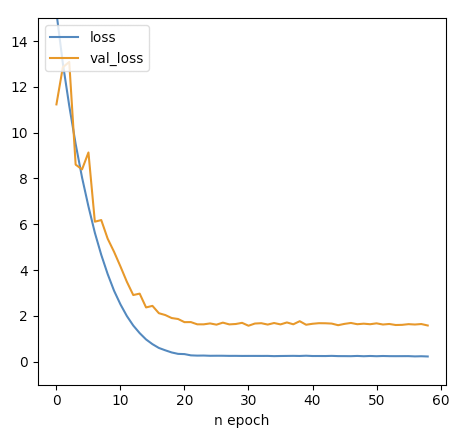
\includegraphics[width=0.3\textwidth]{images/loss.png}
    \caption{Baseline training loss curve}
    \label{fig:loss-curve}
\end{wrapfigure}

\begin{figure}[hbt!]
    \centering
    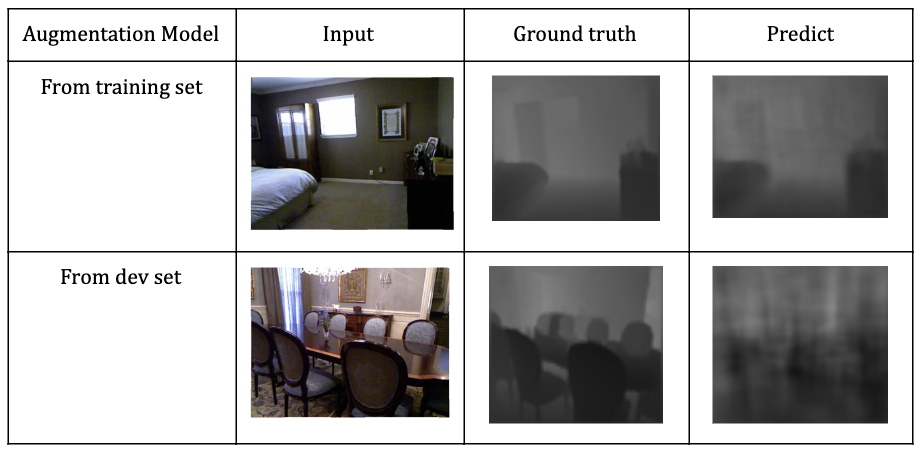
\includegraphics[width=0.8\textwidth]{images/augmented-model-output.png}
    \caption{Output of the data augmented model}
    \label{fig:augmentation-output}
\end{figure}

\section{Metrics}
    We used three metrics to evaluate the performance of each approach as well as compare it with the published results of other methods. 
    
    The notation $\hat{y}$ refers to the predicted depth map and $y$ refers to the ground truth, each with N pixels of i index. $T$ is the number of samples.

\begin{itemize}
    \item Absolute relative difference: $\frac{1}{T}\sum_1^T|y-\hat{y}|/y$
    \item Squared relative difference: $\frac{1}{T}\sum_1^T|y-\hat{y}|^2/y$
    \item Root Mean Squared Error (RMSE): $\sqrt{\frac{1}{T}\sum_1^T|y-\hat{y}|^2}$
\end{itemize}

% Please add the following required packages to your document preamble:
% \usepackage{booktabs}
\begin{table}[]
    \centering
    \begin{tabular}{@{}llllll@{}}
    \toprule
                  & Baseline & Augmentation & Dropout & Regularization & Dropout + Augmentation \\ \midrule
    Abs Rel Diff  & 0.294          & \textbf{0.286}             & 0.272    & 0.318     & 0.309        \\
    Sqrt Rel Diff & 0.391          & \textbf{0.356}             & 0.349    & 0.471     & 0.375        \\
    RMSE          & 1.161          & \textbf{1.076}             & 1.113    & 1.296     & 1.056        \\ \bottomrule
    \end{tabular}
    \caption{Metric of our approach}
    \label{table:1}
\end{table}

% Please add the following required packages to your document preamble:
% \usepackage{booktabs}
\begin{table}[]
    \centering
    \begin{tabular}{@{}llllll@{}}
    \toprule
                  & Make3D & Eigen      & Karsch \\ \midrule
    Abs Rel Diff  & 0.408  & 0.215      & 0.350 \\
    Sqrt Rel Diff & 0.581  & 0.212      & 0.223 \\
    RMSE          & 1.24   & 0.907      & 1.2   \\ \bottomrule
    \end{tabular}
    \caption{Metric of other approaches}
    \label{table:2}
\end{table}

    We saw progressive improvements to the outcome with each approach added to the baseline, except for regularization (see table \ref{table:1}). For our final model, we picked the model with data augmentation as it seemed to perform the best among all the approaches we tried.
    
    Eigen et al was the paper that we based our model on. We managed to achieve results close to theirs but was unable to surpass it. In the next section, we will discuss some potential areas of improvement to our model to achieve better outcomes. (see \ref{conclusion})


\section{Conclusions and Future Work} \label{conclusion}
    From the results, our approach showed very promising results while predicting on datasets that the model has seen before. However it suffers from a large variance problem. Dev set performance has not yet reached train set performance. We concluded that the issue originated from the small dataset that we acquired for the training. To resolve the issue, we would like to augment the dataset with more RGB to RGB-Depth image pairs. Besides the existing data used, NYU also provides 407,024 unlabeled frames. Although the data is unlabeled, the depth image information can still be used by our training pipeline. On top of the additional data, we are also planning to perform data augmentation techniques to the existing dataset. 
    
    We also observed from the predicted depth images that they generally lack sharp edges or smooth transitions. From a high level, the model didn’t learn the plane segmentation well in the process. We could modify the network with more feature extraction layers so that the correlation between planes and depth can be learned. Lee et al \cite{pp4} used convolutions to obtain planar guidance before feeding it to output layers. Additionally we could preprocess the image to segmentation map or edge map, and feed the processed image into the network in the deeper layer to make the edge and planes as stronger features to the network. 

\section{Contribution and Code}
    All team members contributed on the project research, network architecture discussion and error analysis.
    
    The code can be found at: https://github.com/jguoxu/depth-estimation
    
    Xu Guo focused on overall architecture of the project (Keras pipeline, model bring up), data processing and augmentation, and optimizing training performance (speed up training from 1min per-epoch to 7s per-epoch). 
    
    Isha Singhal focused on implementing the two pass model training structure, implementing and analyzing the loss function, regularization and analyzing the metrics. 
    
    Meijiao Png implemented the sequential refined model, added dropout and wrote the metric functions. 

\medskip
\small
\begin{thebibliography}{8}

\bibitem{nyu_dataset} 
\textit{https://cs.nyu.edu/~silberman/datasets}
 
\bibitem{nips-1} 
David Eigen, Christian Puhrsch, Rob Fergus
\textit{Depth Map Prediction from a Single Image using a Multi-Scale Deep Network}.
Curran Associates, Inc., NIPS2014-5539, 2014.

\bibitem{github-repo}
\textit{https://github.com/jguoxu/depth-estimation}

\bibitem{pp1} 
David Eigen, Rob Fergus
\textit{Predicting Depth, Surface Normals and Semantic Labels with a Common Multi-Scale Convolutional Architecture}. 
ICCV, pp.2650-2658 609--616, 2015.

\bibitem{pp2} 
Daniel Stanley Tan, Chih-Yuan Yao, Conrado Ruiz, Jr., and Kai-Lung Hua
\textit{Single-Image Depth Inference Using Generative Adversarial Networks}.
2019 Apr 10. doi: 10.3390/s19071708

\bibitem{pp3} 
Shir Gur, Lior Wolf
\textit{Single Image Depth Estimation Trained via Depth From Defocus Cues}.
The IEEE Conference on Computer Vision and Pattern Recognition (CVPR), 2019, pp. 7683-7692

\bibitem{pp4}
Jin Han Lee, Myung-Kyu Han, Dong Wook Ko, Il Hong Suh 
\textit{From Big to Small: Multi-Scale Local Planar Guidance for Monocular Depth Estimation}

\bibitem{pp5}
Ashutosh Saxena, , Sung H. Chung, and Andrew Y. Ng
\textit{Learning Depth from Single Monocular Images}
NIPS, 2005

\bibitem{pp6}
Daniel Stanley Tan, Chih-Yuan Yao, Conrado Ruiz, Jr., and Kai-Lung Hua 
\textit{Single-Image Depth Inference Using Generative Adversarial Networks}
doi: 10.3390/s19071708, 2019 Apr 10.

\bibitem{pp7}
K. Karsch, C. Liu, S. B. Kang, and N. England. 
\textit{Depth extraction from video using nonparametric sampling.}
TPAMI, 2014
\end{thebibliography}

% \end{multicols}

\end{document}